\documentclass[14pt,border=10pt]{standalone}
\usepackage{tikz}
\usepackage[american]{circuitikz}
\usepackage{textcomp}

\usetikzlibrary{shapes,arrows}

\begin{document}
% Definition of blocks:
\tikzset{%
  block/.style    = {draw, thick, rectangle, align=center, minimum height = 3em, minimum width = 3em},
  blockg/.style    = {draw, thick, rectangle, align=center, minimum height =
3cm, minimum width = 3cm},
  mult/.style      = {draw, circle, node distance = 2cm}, % Adder
  input/.style    = {coordinate}, % Input
  output/.style   = {coordinate} % Output
}
% Defining string as labels of certain blocks.
\newcommand{\suma}{\Large$+$}
\newcommand{\mult}{\Huge x}
\newcommand{\inte}{$\displaystyle \int$}
\newcommand{\derv}{\huge$\frac{d}{dt}$}

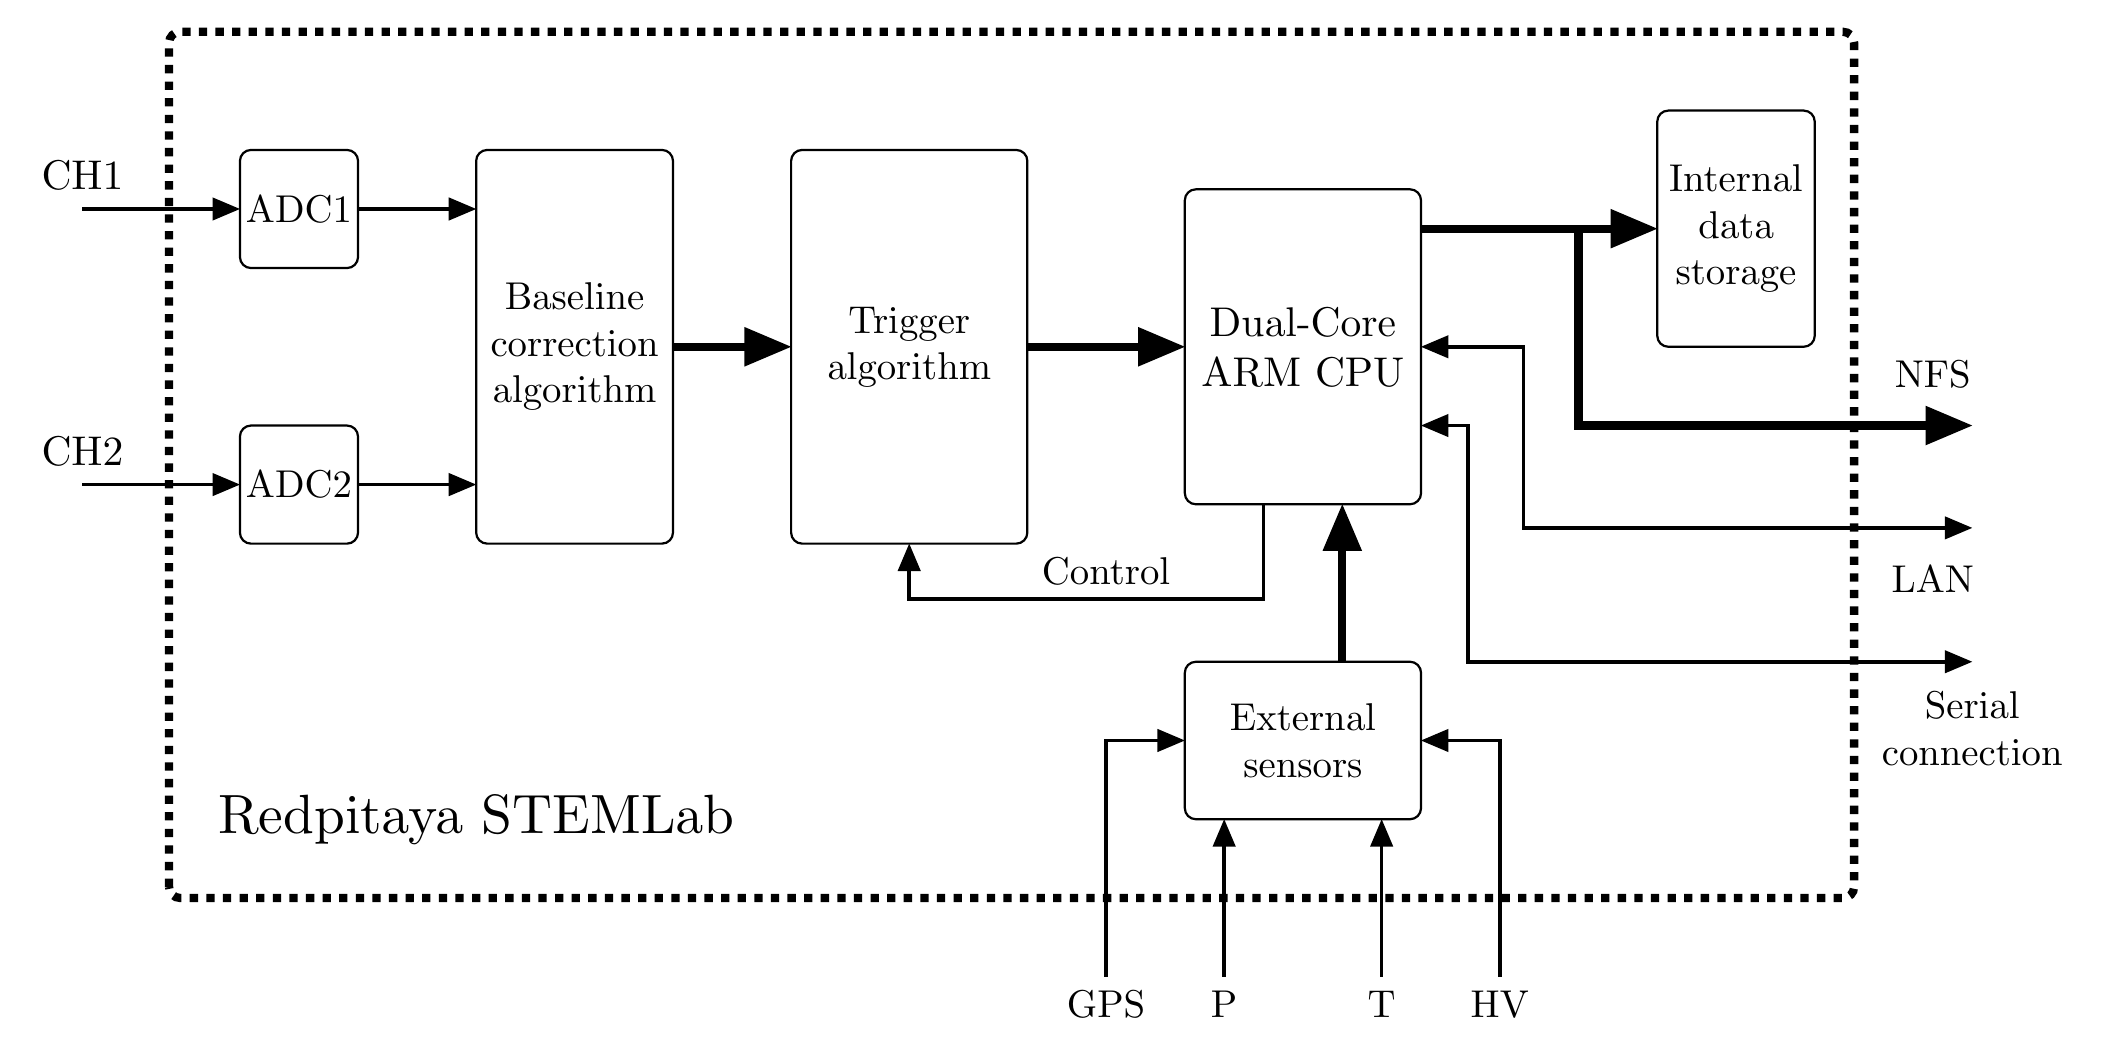
\begin{tikzpicture}[auto, thick, node distance=2cm, >=triangle 45]

%\draw[help lines, ultra thin] (-1,-10) grid (26,10); 
\draw [rounded corners,dashed,line width=3] (1.1,-7) rectangle (22.5,4);
\draw [rounded corners] (2,1) rectangle (3.5,2.5);
\draw [rounded corners] (2,-1) rectangle (3.5,-2.5);
\draw [rounded corners] (5,-2.5) rectangle (7.5,2.5);
\draw [rounded corners] (9,-2.5) rectangle (12,2.5);
\draw [rounded corners] (14,-2) rectangle (17,2);
\draw [rounded corners] (14,-6) rectangle (17,-4);
\draw [rounded corners] (20,0) rectangle (22,3);

%lineas
				\draw [->,line width=1.3] (0,1.75) -- (2,1.75);
				\draw [->,line width=1.3] (0,-1.75) -- (2,-1.75);

				\draw [->,line width=1.3] (3.5,1.75) -- (5,1.75);
				\draw [->,line width=1.3] (3.5,-1.75) -- (5,-1.75);

				\draw [->,line width=3] (7.5,0) -- (9,0);
				\draw [->,line width=3] (12,0) -- (14,0);
				\draw [->,line width=3] (16,-4) -- (16,-2);
				\draw [->,line width=1.3] (15,-2) -- (15,-3.2) -| (10.5, -2.5);
				\draw [->,line width=1.3] (13,-8) |- (14,-5);
				\draw [->,line width=1.3] (14.5,-8) -- (14.5,-6);
				\draw [->,line width=1.3] (16.5,-8) -- (16.5,-6);
				\draw [->,line width=1.3] (18,-8) |- (17,-5);

				\draw [->,line width=3] (17,1.5) -- (20,1.5);
				\draw [->,line width=3] (19,1.5) |- (24,-1);
				\draw [<->,line width=1.3] (17,0) -- (18.3,0) |- (24,-2.3);
				\draw [<->,line width=1.3] (17,-1) -- (17.6,-1) |- (24,-4);

%nodes
				\node [align=center,scale=2] at (5,-6) {Redpitaya STEMLab};
				\node [above=3mm, align=center,scale=1.5] at (0,1.5) {CH1};
				\node [above=-1mm, align=center,scale=1.5] at (0,-1.6) {CH2};
				\node [align=center,scale=1.4] at (2.75,1.75) {ADC1};
				\node [align=center,scale=1.4] at (2.75,-1.75) {ADC2};
				\node [align=center,scale=1.4] at (6.25,0)
				{Baseline\\correction\\algorithm};
				\node [align=center,scale=1.4] at (10.5,0) {Trigger\\algorithm};
				\node [above,align=center,scale=1.4] at (13,-3.2) {Control};
				\node [align=center,scale=1.5] at (15.5,0) {Dual-Core\\ARM CPU};
				\node [align=center,scale=1.4] at (15.5,-5) {External\\sensors};
				\node [below,align=center,scale=1.4] at (13,-8) {GPS};
				\node [below,align=center,scale=1.4] at (14.5,-8) {P};
				\node [below,align=center,scale=1.4] at (16.5,-8) {T};
				\node [below,align=center,scale=1.4] at (18,-8) {HV};
				\node [align=center,scale=1.4] at (21,1.5) {Internal\\data\\storage};
				\node [above=3mm,align=center,scale=1.4] at (23.5,-1) {NFS};
				\node [below=1mm,align=center,scale=1.4] at (23.5,-2.5) {LAN};
				\node [below=2mm,align=center,scale=1.4] at (24,-4) {Serial\\connection};
%\draw 
%  % Drawing the blocks of first filter :
%  node at (0,0)[right=-3.3mm]{\Large \textopenbullet}
%  node at (0,0)[input, name=sigin] {}
%  node at (2,0)[block, right of=sigin] (ad1) {ADC1}
%  node at (8,0) [mixer] (mult1) {}
%  node at (8,-2)[mixer] (mult2) {}
%  node at (0,-4)[right=-3.3mm]{\Large \textopenbullet}
%  node at (0,-4)[input, name=refin] {}
%  node at (0,-4)[block, right of=refin] (ad2) {ADC2}
%  node [block, right of=ad2] (zcd) {ZCD}
%  node [block, right of=zcd] (adpll) {ADPLL}
%  node [block, below of=adpll] (intref) {INT. REF.}
%  node [block, right of=mult1] (lpf1) {LPF}
%  node at (14,-1)[blockg] (soc) {Dual Core\\ARM CPU}
%  node [block, right of=mult2] (lpf2) {LPF}
%  node at (17.6,0)[block] (da1) {DAC1}
%  node at (17.6,-2)[block] (da2) {DAC2};
%
%   % Joining blocks. 
%    % Commands \draw with options like [->] must be written individually
%  \draw[->](sigin) -- node {Sig. In}(ad1);
%  \draw[->](ad1) -- (mult1.west);
%  \draw[->](mult1.east) -- node {} (lpf1);
%  \draw[->](lpf1) -- node {} (12.5,0);
%  \draw[->](refin) -- node {Ref. In} (ad2);
%  \draw[->](ad2) -- node {}(zcd);
%  \draw[->](zcd) -- node {}(adpll);
%  \draw[->](intref) -- node {} (adpll);
%  \draw[->](soc) |- node {} (intref);
%  \draw[->](mult2.east) -- node {} (lpf2);
%  \draw[->](lpf2) -- node {} (12.5,-2);
%  \draw[*-] (4,0.1) -- node {} (4,-2);
%  \draw[->] (4,-2) -- (7.5,-2);
%  \draw[->] (adpll.east) -| node {} (mult2.south);
%  \draw (adpll.north) -- node {} (6,-1);
%  \draw[->] (6,-1) -| node {} (mult1.south);
%  \draw[->] (15.5,0) -- node {} (17,0);
%  \draw[->] (15.5,-2) -- node {} (17,-2);
%  \draw[->] (18.2,0) -- node {Out1} (20,0);
%  \draw[->] (18.2,-2) -- node {Out2} (20,-2);
  
\end{tikzpicture}
\end{document}
